\chapter{A espectroscopia no infravermelho}\label{ch:g11:infrared}

Numa prateleira de laboratório está um frasco de líquido incolor cujo
rótulo foi arrancado. Pode ser um \omterm{def:g11:functional-groups:alcohol}{álcool}, uma \omterm{def:g11:functional-groups:carbonyl}{cetona} ou um ácido: três
famílias que parecem exatamente iguais dentro de um frasco. Uma gota
colocada no cristal de um espectrômetro de infravermelho, dois minutos
de espera, e aparece na tela um gráfico que responde à pergunta. As
ligações de uma \omterm{def:g7:atoms-and-molecules:molecule}{molécula} vibram, e cada tipo de ligação absorve a luz
infravermelha de frequências próprias: um \omterm{def:g11:infrared:spectrum}{espectro infravermelho} é uma
lista das ligações presentes.

\begin{recall}
Os \omterm{def:g11:functional-groups:functional-group}{grupos funcionais} e as famílias (\cref{ch:g11:functional-groups}).
Um \omterm{def:g11:absorbance:spectrum}{espectro de absorção} mostra quanta luz uma substância absorve em cada
comprimento de onda (\cref{ch:g11:absorbance}). As \omterm{def:g11:polarity-and-cohesion:hydrogen-bond}{ligações de
hidrogênio} ligam os grupos \ce{O-H} a \omterm{def:g7:atoms-and-molecules:molecule}{moléculas} vizinhas
(\cref{ch:g11:polarity-and-cohesion}).
\end{recall}

\section{As ligações vibram}

Uma \omterm{def:g10:lewis-and-shape:covalent-bond}{ligação covalente} não é rígida: os dois \omterm{def:g7:atoms-and-molecules:atom}{átomos} vibram, se aproximando
e se afastando muitos milhões de milhões de vezes por segundo, como duas
bolas presas por uma mola. Uma mola mais dura (uma \omterm{def:g10:lewis-and-shape:multiple-bond}{ligação dupla} em vez
de uma simples) ou bolas mais leves (um \omterm{def:g7:atoms-and-molecules:atom}{átomo} de hidrogênio em vez de um
\omterm{def:g7:atoms-and-molecules:atom}{átomo} de carbono) vibram mais depressa. Uma ligação pode absorver uma
luz infravermelha cuja frequência coincide com a da sua vibração: a luz
infravermelha, invisível ao olho, tem comprimentos de onda de alguns
micrômetros a algumas dezenas de micrômetros.

\begin{omfigure}
\begin{tikzpicture}[font=\small]
  \node[aC] (c) at (0,0) {};
  \node[aO] (o) at (2.2,0) {};
  \draw[decorate, decoration={coil, aspect=0.4, segment length=4pt,
    amplitude=4pt}, thick, black!60] (c.east) -- (o.west);
  \draw[<->, omProp, thick] (-0.9,0) -- (-0.45,0);
  \draw[<->, omProp, thick] (2.65,0) -- (3.1,0);
  \node[anchor=north] at (1.1,-0.5) {uma ligação que se estica e se encolhe};
  \node[aO] (o1) at (5.3,0) {};
  \node[aH] (h1) at (6.7,0) {};
  \draw[decorate, decoration={coil, aspect=0.4, segment length=3pt,
    amplitude=3pt}, thick, black!60] (o1.east) -- (h1.west);
  \draw[<->, omProp, thick] (7.0,0) -- (7.7,0);
  \node[anchor=north, align=center] at (6.2,-0.5) {um átomo de hidrogênio leve:\\ vibração mais rápida};
\end{tikzpicture}

{\small Uma ligação representada como uma mola entre duas bolas. A sua
vibração tem uma frequência fixada pela rigidez da ligação e pelas massas
dos \omterm{def:g7:atoms-and-molecules:atom}{átomos}; a luz infravermelha dessa frequência é absorvida.}
\end{omfigure}

\begin{definition}[Número de onda]\label{def:g11:infrared:wavenumber}
O \emph{número de onda}\index{numero de onda@número de onda} $\sigma$ de uma luz é o
inverso do seu comprimento de onda, $\sigma = 1/\lambda$. Em
espectroscopia no infravermelho, ele é expresso em \si{cm^{-1}}: o
número de comprimentos de onda num centímetro. Um número de onda maior
quer dizer um comprimento de onda mais curto e uma vibração mais
rápida.
\end{definition}

\begin{example}[De um número de onda a um comprimento de onda]\label{ex:g11:infrared:convert}
Uma banda em $\sigma = \qty{2000}{cm^{-1}}$ corresponde a
$\lambda = 1/2000 = \qty{5.0e-4}{cm} = \qty{5.0}{\micro m}$. Os \omterm{def:g11:infrared:spectrum}{espectros
infravermelhos} em geral vão de \qty{4000}{cm^{-1}} (\qty{2.5}{\micro m})
a \qty{500}{cm^{-1}} (\qty{20}{\micro m}).
\end{example}

\section{Ler um espectro infravermelho}

\begin{definition}[Espectro infravermelho, transmitância]\label{def:g11:infrared:spectrum}
A \emph{transmitância}\index{transmitancia@transmitância} $T$ de uma amostra num dado
\omterm{def:g11:infrared:wavenumber}{número de onda} é a porcentagem da luz infravermelha que a atravessa:
\qty{100}{\percent} se nada é absorvido. O \emph{espectro
infravermelho}\index{espectro infravermelho} de um composto é o gráfico
de $T$ em função do \omterm{def:g11:infrared:wavenumber}{número de onda}, desenhado por convenção com os
\omterm{def:g11:infrared:wavenumber}{números de onda} diminuindo da esquerda para a direita.
\end{definition}

\begin{definition}[Banda de absorção, região da impressão digital]\label{def:g11:infrared:band}
Uma \emph{banda de absorção}\index{banda de absorcao@banda de absorção} é uma queda da
\omterm{def:g11:infrared:spectrum}{transmitância}: a luz desses \omterm{def:g11:infrared:wavenumber}{números de onda} é absorvida por uma ligação.
A sua posição diz qual é a ligação; a sua largura e a sua profundidade
completam o quadro. Abaixo de cerca de \qty{1500}{cm^{-1}}, o espectro
fica cheio de bandas que dependem da \omterm{def:g7:atoms-and-molecules:molecule}{molécula} inteira: essa \emph{região
da impressão digital}\index{regiao da impressao digital@região da impressão digital} identifica um
composto por comparação com um espectro conhecido, mas é difícil de ler
ligação por ligação.
\end{definition}

\begin{inthelab}[Registrar um espectro]
A maioria dos espectrômetros das escolas e das universidades usa hoje
um pequeno cristal de diamante: uma gota de líquido, ou alguns grãos de
sólido apertados por uma presilha, é colocada sobre o cristal, e o feixe
infravermelho que roça a sua superfície sonda a amostra. Primeiro, o
cristal é registrado limpo (o ``fundo''), que faz o papel do branco. O
cristal é limpo com um lenço de papel e um pouco de \omterm{def:g6:solutions-and-solubility:solute}{solvente} entre duas
amostras.
\end{inthelab}

\section{As bandas características}

\begin{proposition}[Cada tipo de ligação tem a sua banda]\label{prop:g11:infrared:bands}
% ledger: ir:OH-free, ir:OH-bonded, ir:OH-acid, ir:NH, ir:CH, ir:CO-aldehyde, ir:CO-ketone, ir:CO-ester, ir:CO-acid, ir:CC-double, ir:CO-single
Cada tipo de ligação absorve numa faixa característica de \omterm{def:g11:infrared:wavenumber}{números de
onda}, quase a mesma de uma \omterm{def:g7:atoms-and-molecules:molecule}{molécula} para outra:
\begin{center}
\small
\begin{tabular}{lll}
\hline
ligação & n.º de onda (\si{cm^{-1}}) & aspecto \\
\hline
\ce{O-H} sem ligação de H (gás, diluído) & perto de 3600 & fina \\
\ce{O-H} com ligação de H (\omterm{def:g11:functional-groups:alcohol}{álcool} líquido) & 3300--3400 & larga, forte \\
\ce{O-H} de um \omterm{def:g11:functional-groups:carboxylic-acid}{ácido carboxílico} & 2500--3300 & muito larga \\
\ce{N-H} de uma \omterm{def:g11:functional-groups:amine}{amina} & 3300--3500 & média (duas bandas para \ce{-NH2}) \\
\ce{C-H} de uma cadeia & 2850--2960 & forte \\
\ce{C=O} de um \omterm{def:g11:functional-groups:carboxylic-acid}{éster} & perto de 1735 & muito forte, fina \\
\ce{C=O} de um \omterm{def:g11:functional-groups:carbonyl}{aldeído} & perto de 1730 & muito forte, fina \\
\ce{C=O} de uma \omterm{def:g11:functional-groups:carbonyl}{cetona} & perto de 1715 & muito forte, fina \\
\ce{C=O} de um \omterm{def:g11:functional-groups:carboxylic-acid}{ácido carboxílico} & perto de 1710 & muito forte, mais larga \\
\ce{C=C} & perto de 1650 & média \\
\ce{C-O} de um \omterm{def:g11:functional-groups:alcohol}{álcool} & perto de 1050 & forte \\
\hline
\end{tabular}
\end{center}
\end{proposition}

\begin{proof}
Essas faixas são medidas em muitos compostos. Elas
se agrupam por ligação porque a vibração de uma ligação depende
sobretudo da própria ligação e dos seus dois \omterm{def:g7:atoms-and-molecules:atom}{átomos}, e pouco do resto
da \omterm{def:g7:atoms-and-molecules:molecule}{molécula}.
\end{proof}

\begin{omfigure}
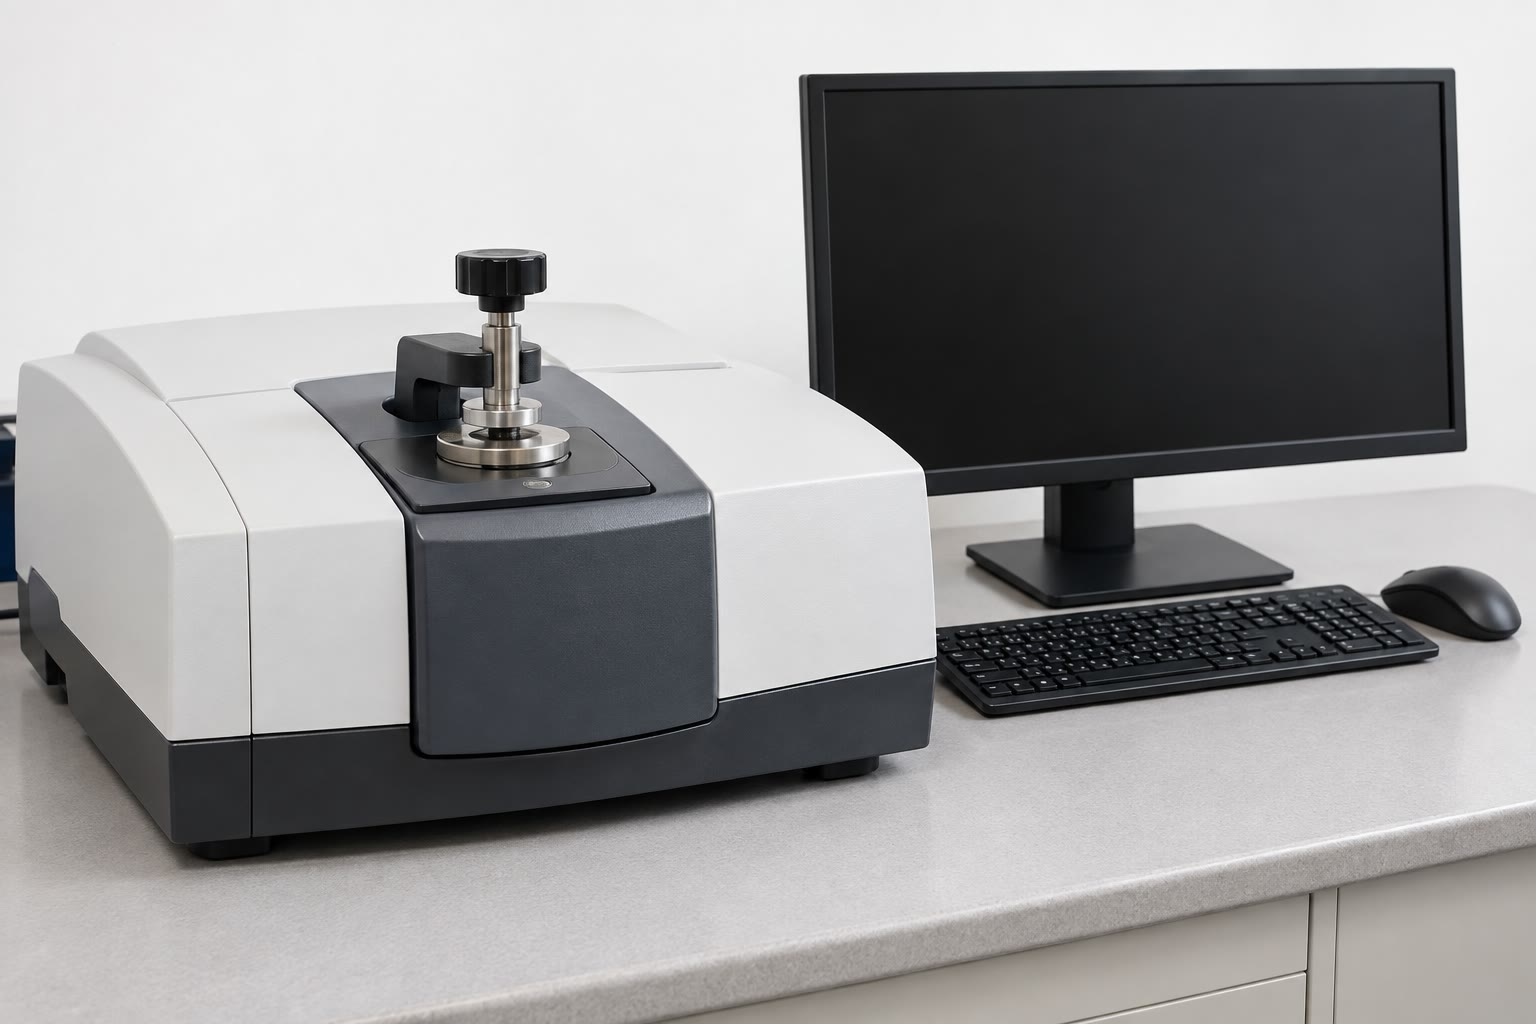
\includegraphics[width=0.48\linewidth]{images/book1/ai/g11-ftir.jpg}

{\small Um espectrômetro de infravermelho de bancada, com o seu cristal e a sua presilha.}
\end{omfigure}

\begin{omfigure}
\begin{tikzpicture}[font=\small, x=0.0036cm, y=0.5cm]
  % wavenumber axis reversed: x = 4000 - sigma
  \fill[black!8] (2500,0.2) rectangle (3500,7.6);
  \node[font=\footnotesize, align=center, black!60] at (3000,6.8) {região da\\ impressão digital};
  \draw[->] (0,0) -- (3600,0) node[right] {$\sigma$};
  \foreach \s in {4000,3500,3000,2500,2000,1500,1000,500}
    \draw ({4000-\s},0) -- ({4000-\s},-0.15) node[below, font=\footnotesize] {\s};
  \node[below=12pt] at (1800,-0.3) {número de onda (\si{cm^{-1}})};
  \foreach \a/\b/\y/\c/\l in {
      3600/3600/7/omDef/{\ce{O-H} livre},
      3300/3400/6/omDef/{\ce{O-H} ligado},
      2500/3300/5/omThm/{\ce{O-H} ácido},
      3300/3500/4/omMeth/{\ce{N-H}},
      2850/2960/3/black!60/{\ce{C-H}},
      1700/1740/2/omProp/{\ce{C=O}},
      1050/1050/1/black!45/{\ce{C-O}}} {
    \fill[\c, rounded corners=1pt] ({4000-\b-12},{\y-0.25}) rectangle ({4000-\a+12},{\y+0.25});
    \node[anchor=west, font=\footnotesize] at ({4000-\a+40},\y) {\l};
  }
\end{tikzpicture}

{\small Onde as principais ligações absorvem. As bandas \ce{O-H} e
\ce{N-H} ficam à esquerda, a banda \ce{C=O}, em geral a mais forte,
perto de \qty{1700}{cm^{-1}}; abaixo de \qty{1500}{cm^{-1}} fica a
\omterm{def:g11:infrared:band}{região da impressão digital}.}
\end{omfigure}

\begin{proposition}[As ligações de hidrogênio alargam a banda O--H]\label{prop:g11:infrared:hbond}
% ledger: ir:OH-free, ir:OH-bonded, ir:ethanol-OH
Quando os grupos \ce{O-H} estão ligados por \omterm{def:g11:polarity-and-cohesion:hydrogen-bond}{ligações de hidrogênio}, como
num \omterm{def:g11:functional-groups:alcohol}{álcool} líquido, a sua banda é larga e fica em \omterm{def:g11:infrared:wavenumber}{números de onda} mais
baixos (cerca de 3300--\qty{3400}{cm^{-1}}); sem \omterm{def:g11:polarity-and-cohesion:hydrogen-bond}{ligações de hidrogênio},
como no gás, ela é fina e fica perto de \qty{3600}{cm^{-1}}.
\end{proposition}

\begin{proof}
Admitido: uma \omterm{def:g11:polarity-and-cohesion:hydrogen-bond}{ligação de hidrogênio} puxa o \omterm{def:g7:atoms-and-molecules:atom}{átomo} de hidrogênio e afrouxa
a ligação \ce{O-H}, que vibra mais devagar; e como cada \omterm{def:g7:atoms-and-molecules:molecule}{molécula} está
ligada de um jeito um pouco diferente, a banda se espalha por uma faixa.
\end{proof}

\section{Identificar os grupos funcionais}


\begin{method}[Ler um espectro infravermelho]\label{met:g11:infrared:reading}
\begin{enumerate}
  \item Olhe primeiro acima de \qty{1500}{cm^{-1}}; deixe a \omterm{def:g11:infrared:band}{região da
        impressão digital} para uma comparação com espectros conhecidos.
  \item Perto de \qty{1700}{cm^{-1}}: uma banda muito forte indica um
        grupo \ce{C=O} (\omterm{def:g11:functional-groups:carbonyl}{aldeído}, \omterm{def:g11:functional-groups:carbonyl}{cetona}, ácido, \omterm{def:g11:functional-groups:carboxylic-acid}{éster}, \omterm{def:g11:functional-groups:amine}{amida}).
  \item Entre 2500 e \qty{3700}{cm^{-1}}: uma banda larga perto de
        \qty{3350}{cm^{-1}} indica um \ce{O-H} de \omterm{def:g11:functional-groups:alcohol}{álcool}; uma banda muito
        larga de 2500 a \qty{3300}{cm^{-1}} com um \ce{C=O} indica um
        \omterm{def:g11:functional-groups:carboxylic-acid}{ácido carboxílico}; bandas médias em 3300--\qty{3500}{cm^{-1}}
        indicam \ce{N-H}.
  \item Combine com a \omterm{def:g11:organic-skeletons:formulas}{fórmula molecular} para escolher a família, e
        depois confira com a posição da banda \ce{C=O}, se houver uma.
\end{enumerate}
\end{method}

\begin{omfigure}
\newcommand{\irpanel}[2]{%
\begin{tikzpicture}
\begin{axis}[width=0.96\linewidth, height=3.9cm, x dir=reverse, xmin=500,
    xmax=4000, ymin=0, ymax=105, xtick={4000,3000,2000,1000},
    /pgf/number format/1000 sep={},
    ytick={0,50,100}, tick label style={font=\scriptsize},
    label style={font=\scriptsize}, ylabel={$T$ (\%)}, axis lines*=left,
    title={\small #2}, title style={yshift=-4pt}]
  \addplot[thick, omDef] table[x=sigma, y=#1] {figdata/out/grade-11-infrared.dat};
\end{axis}
\end{tikzpicture}}
\begin{minipage}{0.49\linewidth}\irpanel{ethanolL}{A: etanol (líquido)}\end{minipage}\hfill
\begin{minipage}{0.49\linewidth}\irpanel{ethanolG}{B: etanol (gás)}\end{minipage}

\begin{minipage}{0.49\linewidth}\irpanel{propanone}{C: propanona}\end{minipage}\hfill
\begin{minipage}{0.49\linewidth}\irpanel{acid}{D: ácido etanoico}\end{minipage}

\begin{minipage}{0.49\linewidth}\irpanel{ester}{E: etanoato de etila}\end{minipage}\hfill
\begin{minipage}{0.49\linewidth}\irpanel{amine}{F: etanamina}\end{minipage}

{\small \omterm{def:g11:infrared:spectrum}{Espectros infravermelhos} de seis compostos, \omterm{def:g11:infrared:wavenumber}{número de onda} em
\si{cm^{-1}} (diminuindo para a direita). Só as bandas discutidas no
capítulo estão desenhadas; as suas posições vêm de espectros medidos e
de tabelas, as suas formas de um modelo simples.}
\end{omfigure}

\begin{example}[Ler os seis espectros]\label{ex:g11:infrared:six}
% ledger: ir:OH-bonded, ir:ethanol-OH, ir:CO-ketone, ir:OH-acid, ir:CO-acid, ir:CO-ester, ir:ethylethanoate-COC, ir:NH
O etanol (A) mostra uma banda \ce{O-H} larga perto de
\qty{3350}{cm^{-1}}, as bandas \ce{C-H} logo abaixo de
\qty{3000}{cm^{-1}} e uma banda \ce{C-O} forte perto de
\qty{1050}{cm^{-1}}, mas nada perto de \qty{1700}{cm^{-1}}. No gás (B), a
sua banda \ce{O-H} vira uma linha fina em \qty{3666}{cm^{-1}}. A
propanona (C) não tem banda \ce{O-H}, mas tem um \ce{C=O} muito forte em
\qty{1715}{cm^{-1}}. O ácido etanoico (D) mostra os dois: uma enorme
banda \ce{O-H} de 2500 a \qty{3300}{cm^{-1}} e um \ce{C=O} em
\qty{1710}{cm^{-1}}. O etanoato de etila (E) tem o seu \ce{C=O} em
\qty{1735}{cm^{-1}} e um \ce{C-O} forte perto de \qty{1240}{cm^{-1}}, e
nenhum \ce{O-H}. A etanamina (F) mostra duas bandas \ce{N-H} médias
acima de \qty{3300}{cm^{-1}}.
\end{example}

\section{Exercícios}

\begin{exercise}[$\star$]\label{exo:g11:infrared:1}
Converta num comprimento de onda em micrômetros:
$\sigma = \qty{3300}{cm^{-1}}$
e $\sigma = \qty{1050}{cm^{-1}}$. Qual corresponde à vibração mais
rápida?
\end{exercise}

\begin{exercise}[$\star$]\label{exo:g11:infrared:2}
Um comprimento de onda de \qty{10}{\micro m} é absorvido. Dê o \omterm{def:g11:infrared:wavenumber}{número de
onda} em \si{cm^{-1}}.
\end{exercise}

\begin{exercise}[$\star$]\label{exo:g11:infrared:3}
Que ligação absorve: perto de \qty{1715}{cm^{-1}}; perto de
\qty{3350}{cm^{-1}} (larga); entre 2850 e \qty{2960}{cm^{-1}}?
\end{exercise}

\begin{exercise}[$\star$]\label{exo:g11:infrared:4}
No espectro C (propanona), encontre a banda mais forte. A que ligação
ela pertence?
\end{exercise}

\begin{exercise}[$\star$]\label{exo:g11:infrared:5}
Por que um \omterm{def:g11:infrared:spectrum}{espectro infravermelho} é desenhado com um eixo de
\omterm{def:g11:infrared:spectrum}{transmitância}, com as bandas apontando para baixo? O que quer dizer
$T = \qty{100}{\percent}$?
\end{exercise}

\begin{exercise}[$\star\star$]\label{exo:g11:infrared:6}
Um composto \ce{C4H8O} mostra uma banda muito forte em
\qty{1715}{cm^{-1}} e nenhuma banda acima de \qty{3000}{cm^{-1}}. Outro,
\ce{C4H10O}, mostra uma banda larga perto de \qty{3350}{cm^{-1}} e
nenhuma perto de \qty{1700}{cm^{-1}}. A que famílias eles pertencem?
Proponha um nome para cada um.
\end{exercise}

\begin{exercise}[$\star\star$]\label{exo:g11:infrared:7}
Explique por que a banda \ce{O-H} do ácido etanoico é tão larga, mais
larga até que a do etanol líquido.
\end{exercise}

\begin{exercise}[$\star\star$]\label{exo:g11:infrared:8}
Compare os espectros A e B do etanol. O que muda, e por quê?
\end{exercise}

\begin{exercise}[$\star\star$]\label{exo:g11:infrared:9}
O propanal e a propanona são os dois \ce{C3H6O}. Os dois mostram uma
banda \ce{C=O} forte. O infravermelho consegue distingui-los só por essa
banda? O que mais poderia ajudar?
\end{exercise}

\begin{exercise}[$\star\star$]\label{exo:g11:infrared:10}
Um composto mostra uma banda forte em \qty{1735}{cm^{-1}}, uma banda
forte perto de \qty{1240}{cm^{-1}} e nada acima de
\qty{3000}{cm^{-1}}. A sua fórmula é \ce{C4H8O2}. Que família? O ácido
etanoico é uma possibilidade? E o ácido butanoico?
\end{exercise}

\begin{exercise}[$\star\star$]\label{exo:g11:infrared:11}
Com qual dos seis espectros uma \omterm{def:g7:atoms-and-molecules:molecule}{molécula} de propan-1-ol mais se
pareceria? E uma de ácido propanoico? Explique.
\end{exercise}

\begin{exercise}[$\star\star\star$]\label{exo:g11:infrared:12}
O propan-2-ol pode ser oxidado a propanona. Uma aluna acompanha a reação
registrando espectros de amostras retiradas a cada dez minutos. Descreva
como os espectros mudam. Como ela sabe que a reação está completa?
\end{exercise}

\begin{exercise}[$\star\star\star$]\label{exo:g11:infrared:13}
O ácido butanoico e o etanoato de etila são \omterm{def:g11:organic-skeletons:isomer}{isômeros}, \ce{C4H8O2}.
Descreva duas diferenças entre os seus \omterm{def:g11:infrared:spectrum}{espectros infravermelhos}, e
explique-as.
\end{exercise}

\begin{exercise}[$\star\star\star$]\label{exo:g11:infrared:14}
Uma amostra de etanoato de etila mostra, além das bandas esperadas, uma
banda larga e fraca perto de \qty{3350}{cm^{-1}}. Sugira duas impurezas
que poderiam causá-la (pense em como os \omterm{def:g11:functional-groups:carboxylic-acid}{ésteres} são produzidos, e no
\omterm{def:g4:air-a-mixture-of-gases:air}{ar}). Como a amostra poderia ser verificada?
\end{exercise}

\begin{exercise}[$\star\star\star$]\label{exo:g11:infrared:15}
A banda \ce{C=O} das \omterm{def:g11:functional-groups:carbonyl}{cetonas} fica perto de \qty{1715}{cm^{-1}}, a de um
\ce{C=C} perto de \qty{1650}{cm^{-1}}, e a banda \ce{C-O} perto de
\qty{1050}{cm^{-1}}. Usando a imagem das duas bolas presas por uma mola,
explique por que uma \omterm{def:g10:lewis-and-shape:multiple-bond}{ligação dupla} \ce{C=O} vibra mais depressa que uma
ligação simples \ce{C-O}. Por que as bandas \ce{O-H}, \ce{N-H} e
\ce{C-H} ficam todas em \omterm{def:g11:infrared:wavenumber}{números de onda} altos?
\end{exercise}

\section{Problema: três frascos sem rótulo}

\begin{problem}[{Problema de fim de semana --- três frascos perderam os
rótulos: qual é qual, e que comprimento de onda a cetona absorve mais?}]
\label{pb:g11:infrared:1}
% ledger: ir:OH-bonded, ir:OH-acid, ir:CO-ketone, ir:CO-acid, ir:CO-single
Três frascos de líquido incolor perderam os rótulos. A lista do estoque
diz que eles contêm etanol, propanona e ácido etanoico. Os seus espectros
são registrados: o frasco 1 dá um espectro como o A, o frasco 2 como o
D, o frasco 3 como o C.

\medskip
\noindent\textbf{Parte I --- Os candidatos.}
\begin{enumerate}
  \item Escreva as \omterm{def:g11:organic-skeletons:formulas}{fórmulas estruturais condensadas} do etanol, da
        propanona e do ácido etanoico.
  \item Dê as suas \omterm{def:g11:organic-skeletons:formulas}{fórmulas moleculares}.
  \item Dê o nome do \omterm{def:g11:functional-groups:functional-group}{grupo funcional} de cada um.
  \item Que ligações de cada um deveriam dar uma banda acima de
        \qty{1500}{cm^{-1}}?
\end{enumerate}

\medskip
\noindent\textbf{Parte II --- Os espectros.}
\begin{enumerate}[resume]
  \item Frasco 1: há uma banda \ce{C=O}? Uma banda \ce{O-H}? Que composto
        é?
  \item Frasco 2: descreva as suas duas características mais fortes. Que
        composto?
  \item Frasco 3: que composto? Que banda decide?
  \item O cheiro poderia tê-los distinguido? Por que é melhor não tentar?
  \item Por que a banda \ce{O-H} do frasco 2 é mais larga que a do
        frasco 1?
\end{enumerate}

\medskip
\noindent\textbf{Parte III --- \omterm{def:g11:organic-skeletons:isomer}{Isômeros}.}
\begin{enumerate}[resume]
  \item O metoximetano é um \omterm{def:g11:organic-skeletons:isomer}{isômero} do etanol. Escreva a sua fórmula. Que
        banda do etanol faltaria no seu espectro?
  \item O propanal é um \omterm{def:g11:organic-skeletons:isomer}{isômero} da propanona. Que banda eles têm em
        comum? Onde ela fica para cada um?
  \item O metanoato de metila, \ce{HCOO-CH3}, é um \omterm{def:g11:organic-skeletons:isomer}{isômero} do ácido
        etanoico. Que banda do ácido faltaria? Onde ficaria a sua banda
        \ce{C=O}?
  \item Por que uma \omterm{def:g11:organic-skeletons:formulas}{fórmula molecular} sozinha não consegue identificar um
        composto, enquanto a fórmula e o espectro juntos em geral
        conseguem?
\end{enumerate}

\medskip
\noindent\textbf{Parte IV --- O comprimento de onda.}
\begin{enumerate}[resume]
  \item Qual é o \omterm{def:g11:infrared:wavenumber}{número de onda} da banda mais forte da propanona?
  \item Expresse-o em \si{m^{-1}}.
  \item Calcule o comprimento de onda absorvido, em metros, e depois em
        micrômetros.
  \item Essa luz é visível? A que tipo de radiação ela pertence?
  \item Faça o mesmo para a banda \ce{C-O} do etanol perto de
        \qty{1050}{cm^{-1}}.
  \item Qual das duas ligações vibra mais depressa?
  \item Dê a resposta final: que comprimento de onda a ligação \ce{C=O}
        da propanona absorve com mais intensidade?
\end{enumerate}
\end{problem}
